\documentclass[12pt]{article}

\usepackage[T1]{fontenc}
\usepackage[polish]{babel}
\usepackage[utf8]{inputenc}
\usepackage{graphicx}
\usepackage{booktabs}
\usepackage{hhline}
\usepackage{multirow}
\usepackage{subfig}
\usepackage{hyperref}

\author{Maciej \textsc{Złotorowicz}}
\title{\textbf{Klasyfikacja na danych \linebreak Climate Model Simulation}}
\date{05.01.2023}

\def\code#1{\texttt{#1}}

\pagenumbering{roman} 

\begin{document}
    \maketitle
    \newpage


    \begin{abstract}
        Projekt dotyczy zbioru danych \code{ climate\_model\_sim\_crashes }. Zawiera on \textbf{540} rekordów z \textbf{21} 
        cechami a zadaniem jest klasyfikacja binarna. 
        

        Zbiór danych posiada kilka charakterystycznych cech - jest on bardzo niezbalansowany a cechy są od siebie całkowicie niezalezne.
        sprawia to że wiele algorytmów klasyfikacji nie radzi sobie z tym zbiorem danych a wiele technik - na przykład redukcji
        wymiarowości PCA czy trenowanie nienadzorowane się tutaj nieprzydadzą.  

        Został wybrany ten zbiór danych właśnie ze względu na te utrudnienia.

        Zostały tutaj zastosowane podstawowe algorytmy klasyfikacji binarnej - regresja logistyczna, drzewa decyzyjne, 
        maszyny wektorów nośnych sieci neuronowe ale z bardzo silną regularyzacją. 
    \end{abstract}
    
    \newpage

    \section{Przegląd danych}
        % image resources/scatter.png
        \begin{figure}[h!]
            \centering
            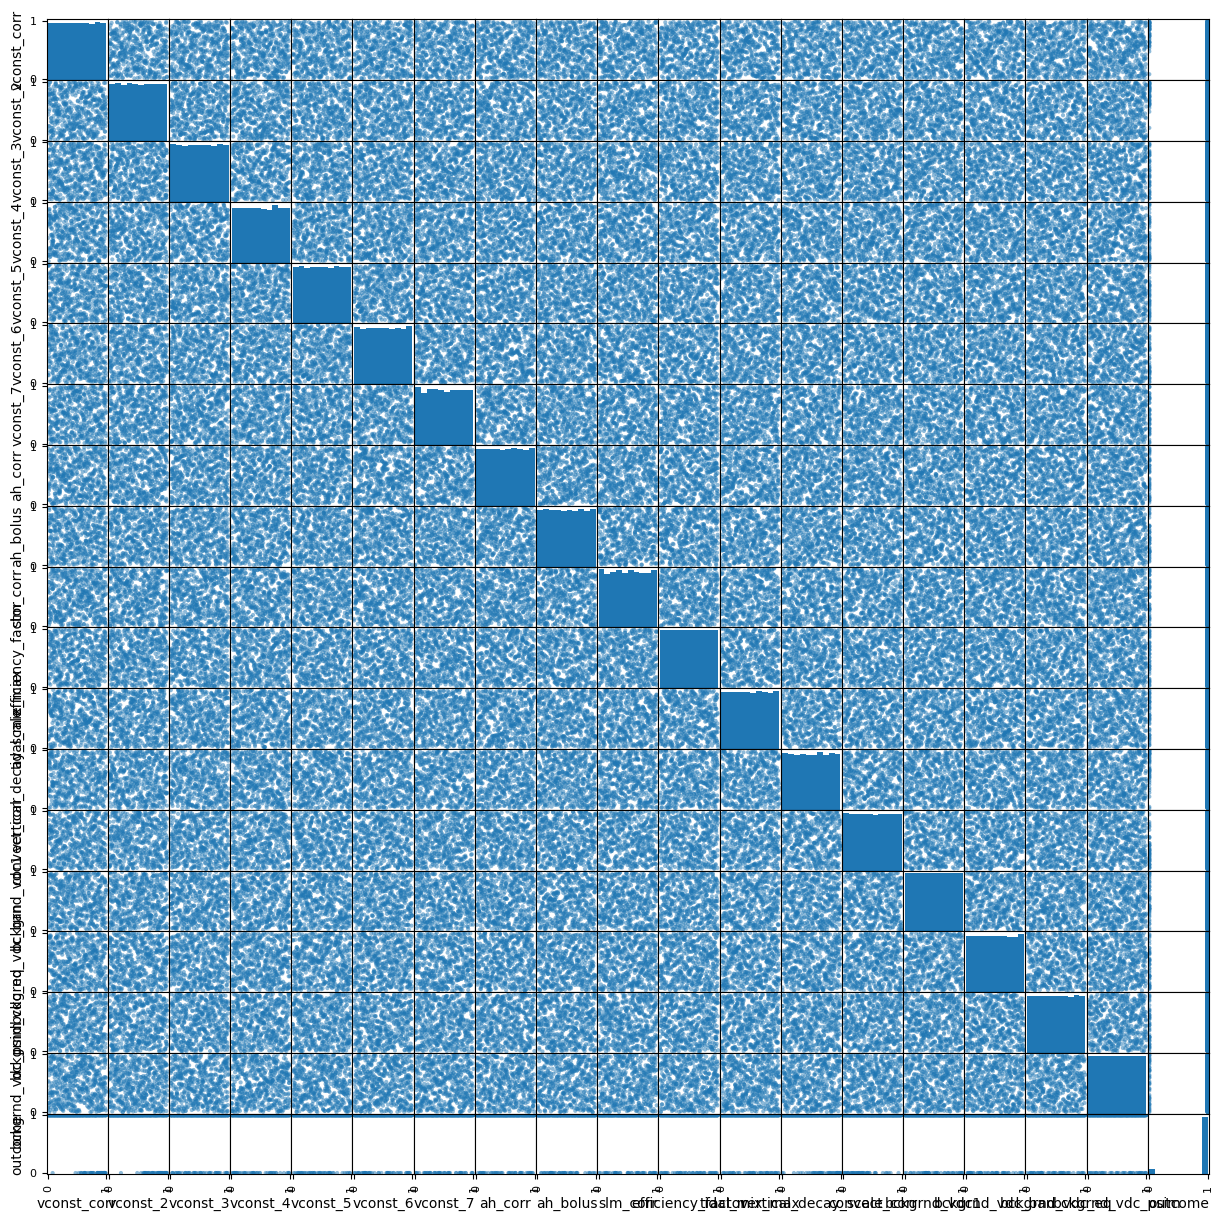
\includegraphics[width=\textwidth]{resources/scatter.png}
            \caption{Rozkład danych}
            \label{fig:scatter}
        \end{figure}

        Pierwszą rzeczą jaką zauważamy na wykresie \ref{fig:scatter} jest to że cechy są od siebie całkowicie niezależne.
        Uniemożliwi to redukcję wymiarowości 
        
        Analizując postawowe parametry statystczne danych możemy zauważyć że dane są bardzo niezbalansowane - 
        średnia z kolumny \code{outcome} wynosi \textbf{0.1}. co oznacza że $90\%$ danych to \code{0} a jedynie $10\%$ to \code{1}
        
        % image resources/corr.png
        \begin{figure}[h!]
            \centering
            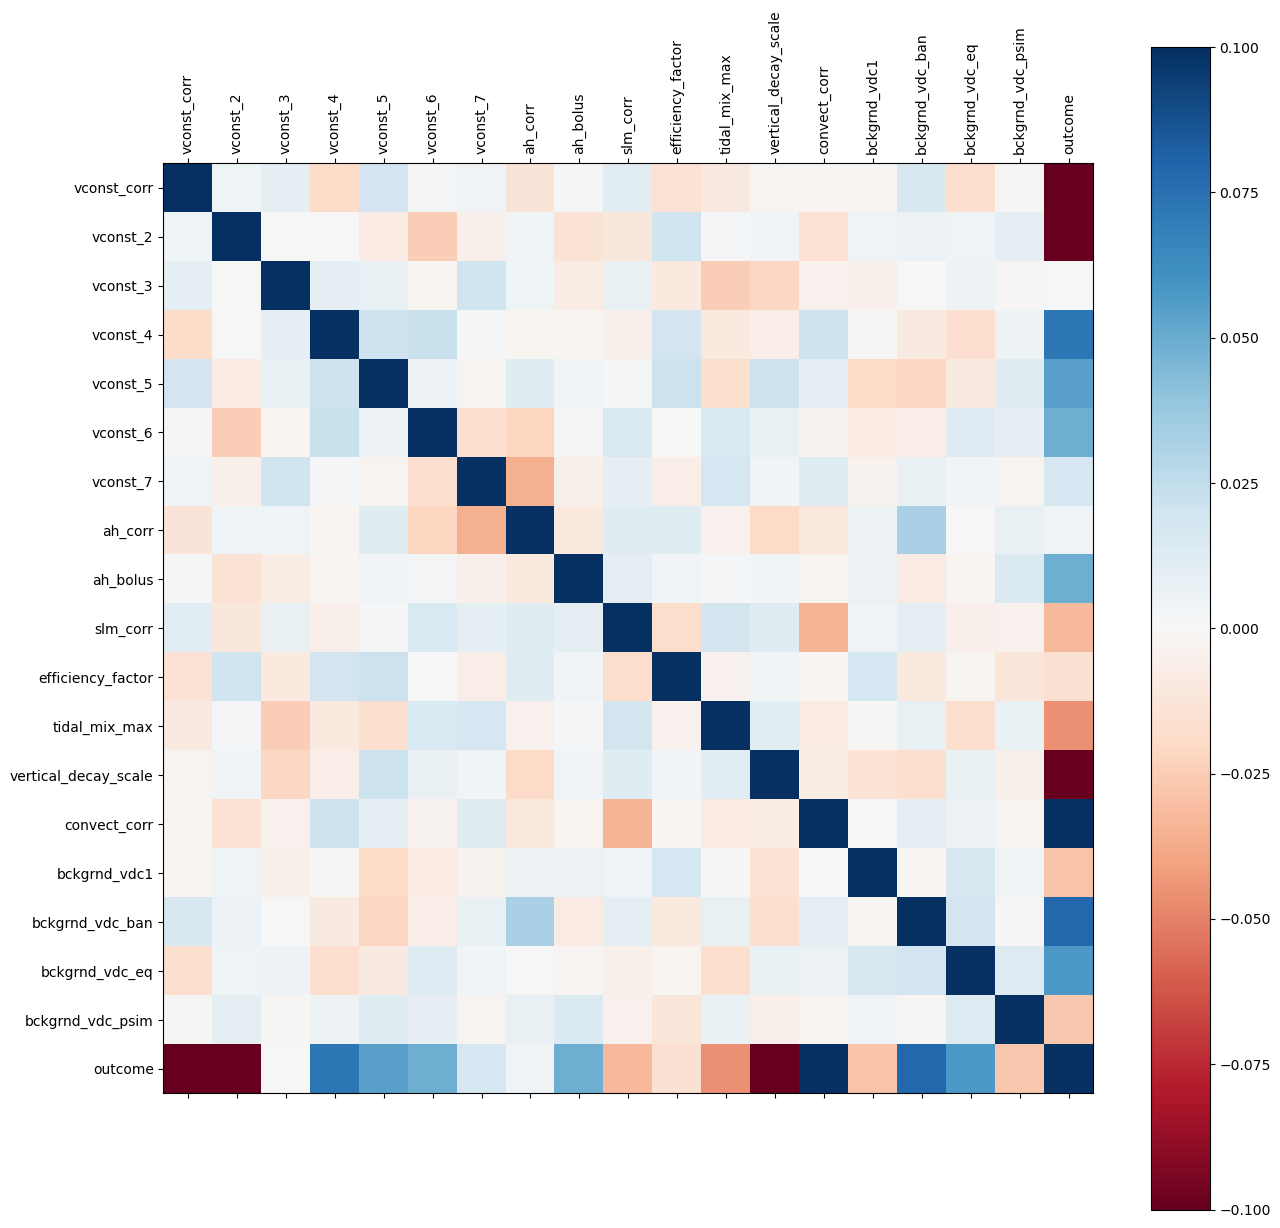
\includegraphics[width=\textwidth]{resources/corr.png}
            \caption{Macierz korelacji}
            \label{fig:corr}
        \end{figure}

        Na szczęscie macierz korelacji pokazuje że cechy są rzeczywiście zależne od \code{outcome} czego nie widać na wykresie \ref{fig:scatter} 
        ponieważ \code{outcome} posiada jedynie dwa unikalne wartości.
        
        \newpage

        \section{Walidacja Modeli}
        W notatniku została przygotowana funkcja która jest użyta do walidowania modeli. Zostały tam wybrane niektóre metryki przedewszystkim:
        \begin{itemize}
            \item Accuracy
            \item Precision
            \item Recall
            \item R2
            \item ROC AUC
        \end{itemize}

        Metryką naważniejszą okazały sie \code{R2} i \code{ROC AUC} ponieważ \code{Accuracy} jest bardzo łatwo osiągalna przez 
        modele i nie nadaje się do oceny ich jakości. Dodatkwo, przez dość małą ilość próbek metryki te są bardzo niestabilne
        Różnica nawet jednej próbki może zmienić wynik o kilkanaście procent w przypadku metryki R2 więc dodatkowo zostały załączone 
        Metryki True Positive Rate i False Positive Rate i macierz pomyłek zarówno dla zbioru uczącego, testowego jak i zbalansowanego.

        \section{Użyte algorytmy i techniki}
        Aby poradzić sobie z tym problemem zostały przetestowane następujące algorytmy i techniki:

        \begin{itemize}
            \item Podstaowa regresja logistyczna
            \item Trenowanie na zbalansowanym podzbiorze
            \item Trenowanie na ważonym zbiorze
            \item Maszyny wektorów nośnych
            \item Polynomial Features
            \item Drzewa decyzyjne
            \item Regularyzowane sieci neuronowe
        \end{itemize}

        Do dobierania parametrów zostało użyte narzędzie \code{GridSearchCV} z biblioteki \code{scikit-learn}. Pozwala ono na 
        przetestowanie wszystkich kombinacji parametrów i wybranie najlepszej z nich. Pozwoliło to szybko odfiltrować klasyfikatory
        które nie nadawały się do tego problemu - drzewa decyzyjne i generowanie cech wielomianowych. Dodatkowo pozwoliło to znaleść
        optymalne parametry dla SVM. Podczas eksperymentowania z sieciami neuronowymi również został użyte przeszukiwanie hiperparametrów
        ale bez skutku. Klasyfikatory które osiągneły słabe wyniki nawet w porównaniu do regresji logistycznej zostały zignorowane.
        
        \subsection{Przeszukiwanie hiperparametrów}
        Aby znaleść dobre klasyfikatory została zdefiniowana przestrzeń parametrów dla klasyfikatorów

        \begin{itemize}
            \item Regresja logistyczna
            \item Extra Trees Classifier
            \item Random Forest Classifier
            \item SVC
        \end{itemize}

        Wyniki przeszukiwania pokazały że jedynie model SVC z kernelm \code{linear} lub \code{rbf} osiągnął dobre wyniki.
        drzewa decyzyjne znalazły się wśród najlepszych ale nie osiągnęły wyników na poziomie SVM dlatego nie były dalej rozpatrywane

        Została również wykonana cross-walidacja aby sprawdzić czy wyniki są stabilne. Modele SVM były niestabline, ale 
        modele sieci neuronowych dawały raczej powtarzalne wyniki.

        \subsection{Sieci neuronowe}

        Klasyfikatory neuronowe zostały najpierw wstępnie przetestowane z różnymi architekturami:

        \begin{itemize}
            \item Wielowarstwowy klasyfikator z \code{Softmax} \newline na końcu i funkcją straty \code{sparse\_categorical\_crossentropy} 
            \item Wielowarstwowy klasyfikator z \code{Sigmoid} \newline na końcu i funkcja straty \code{binary\_crossentropy} 
            \item Dropout na warstwach ukrytych
            \item Regularyzacja L1 i L2 na warstwie wejściowej
            \item Regularyzacja wyjścia inna inicjalizacja biasu
            \item Ważenie próbek wejściowych
        \end{itemize}

        Ostatecznie architektura zatrzymała się na trzech warstwach po 32 neurony, dropout 0.5, early stopping i funkcja aktywacji ELU.

        Do uczenia zostały użyte sztuczki z tej strony \href{http://karpathy.github.io/2019/04/25/recipe/#2-set-up-the-end-to-end-trainingevaluation-skeleton--get-dumb-baselines}{link}

        \section{Wyniki Klasyfikacji}

        Ogólnie bardzo dobrze poradziły sobie maszyny wektorów nośnych i sieci neuronowe, prawdopodobnie obie techniki 
        osiągneły maksymalny możliwy wynik R2 i AUC. Regresja logistyczna i drzewa decyzyjne osiągnęły wyniki owiele gorsze. 

        Szczegółowe wyniki można znaleść w notatniku \code{projekt.ipynb}. Tutaj zostaną przedstawione jedynie wybrane wyniki.

        Na tabeli poniżej widac wszystkie modele które uzyskały w jakiś sposób satysfakcjonujący wynik, zazwyczaj oznaczało to
        wysoki wpsółczynnik $R^2$ i $AUC$, ale nie zawsze. W zależności od wymagań, można na przykład wybrać model generujacy większą 
        dokładność danych albo model który ma większą pełność.

        \begin{itemize}
            \item \code{recall} - pełność
            \item \code{pre} - prezycja
            \item \code{acc} - dokładność
            \item \code{r2} - współczynnik determinacji
        \end{itemize}

        \newpage

        % create table with results, columns metrics, rows models
        \begin{table}[ht!]
            \centering
            \begin{tabular}{lcccccccccc}
        \toprule
                              &\multicolumn{2}{c}{recall} & \multicolumn{2}{c}{pre} & \multicolumn{2}{c}{acc} & \multicolumn{2}{c}{r2} \\
                              &val         & train        & val       & train       & val       & train       & val       & train      \\
        \midrule               
        Logistic Reg.         & 1          & 1            & 0.92      & 0.93        & 0.92      & 0.93        & 0.06      & 0.18       \\ 
        Logistic train bal.   & 0.88       & 0.91         & 0.80      & 0.93        & 0.84      & 0.92        & 0.36      & 0.78       \\   
        SVM                   & 0.99       & 0.99         & 0.97      & 0.97        & 0.96      & 0.97        & 0.60      & 0.65       \\   
        SVM on balanced       & 1          & 1            & 0.75      & 0.79        & 0.84      & 0.86        & 0.36      & 0.50       \\   
        SVM weighted          & 0.90       & 0.91         & 1         & 0.99        & 0.91      & 0.91        &-0.09      &-0.09       \\   
        SVM w. on bal.        & 0.77       & 0.86         & 0.87      & 0.95        & 0.84      & 0.91        & 0.36      & 0.72       \\  
        NN                    & 0.97       & 0.98         & 0.97      & 0.97        & 0.96      & 0.96        & 0.53      & 0.55       \\  
        NN on balanced        & 0.88       & 0.97         & 0.72      & 0.80        & 0.78      & 0.86        & 0.15      & 0.56       \\  
        NN biased             & 0.97       & 0.98         & 0.99      & 0.98        & 0.96      & 0.97        & 0.60      & 0.65       \\  
        NN b. on balaced      & 0.88       & 0.97         & 0.72      & 0.83        & 0.78      & 0.89        & 0.15      & 0.67       \\  
        NN weighted           & 0.97       & 0.99         & 0.99      & 0.98        & 0.97      & 0.97        & 0.68      & 0.69       \\  
        NN w. on balaced      & 0.88       & 0.97         & 0.72      & 0.83        & 0.78      & 0.89        & 0.15      & 0.67       \\  
        Only ones             & 1          & 1            & 0.91      & 0.91        & 0.91      & 0.91        &-0.09      &-0.09       \\
        Perfect               & 1          & 1            & 1         & 1           & 1         & 1           &1          & 1          \\
        
        \bottomrule
                \end{tabular}
        \end{table}
        
        Metryką na którą najbardziej zwracałem uwagę był $R^2$, ponieważ jest ona odporna na niezbalansowanie danych, 
        ROC i AUC okazał się również dobrą metryką do przedwczesnego zatrzymywania uczenia. Ze względu na trudność problemu
        trzeba pujść na kompromis między dokładnością a pełnością.
        
        \newpage

        \newpage

        \subsection{Macierze pomyłek}

        % image conf_logistic_regr.png
        \begin{figure}[ht!]
            \centering
            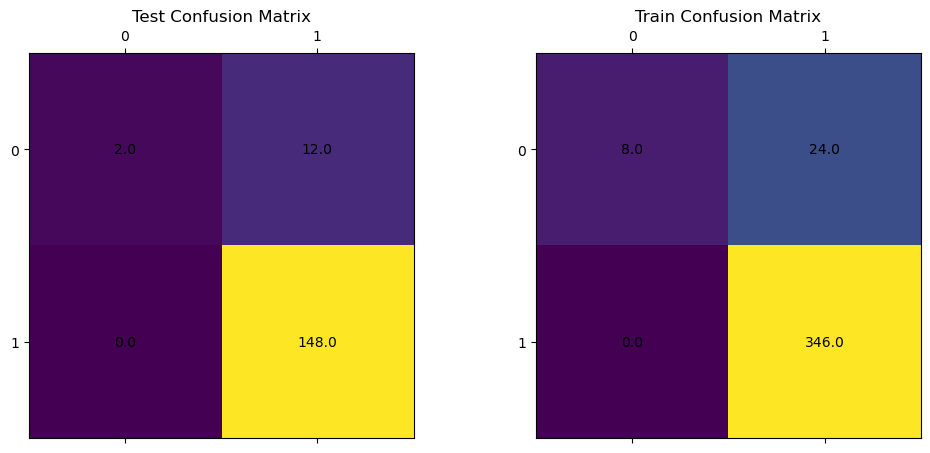
\includegraphics[width=0.9\textwidth]{resources/conf_logistic_regr.png}
            \caption{Logistic Reg.}
            \label{fig:conf_logistic_regr}
        \end{figure}

        % image conf_logistic_regr_on_balanced.png

        \begin{figure}[h!]
            \centering
            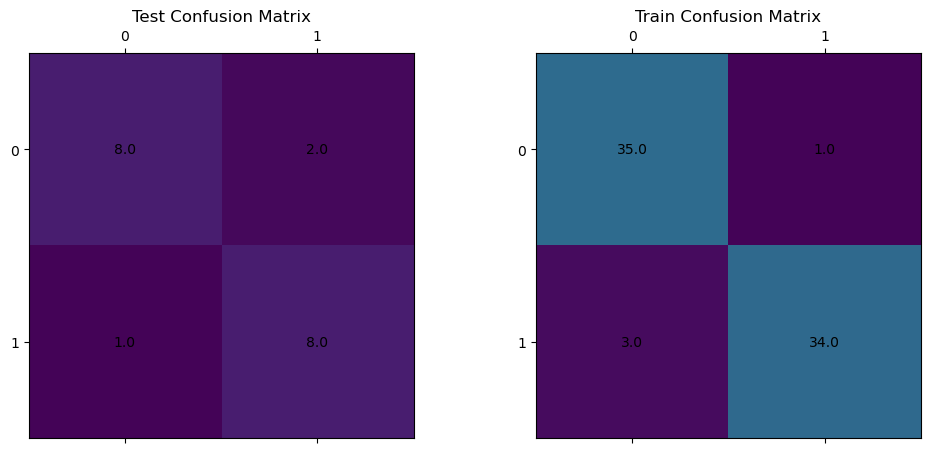
\includegraphics[width=0.9\textwidth]{resources/conf_logistic_regr_on_balanced.png}
            \caption{Logistic Reg. on balanced}
            \label{fig:conf_logistic_regr_on_balanced}
        \end{figure}

        \newpage

        % image conf_svm.png

        \begin{figure}[h!]
            \centering
            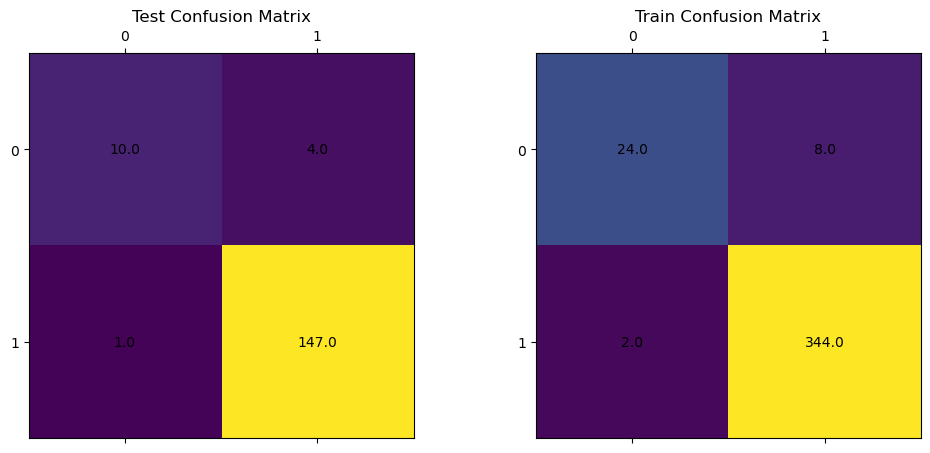
\includegraphics[width=0.9\textwidth]{resources/conf_svm.png}
            \caption{SVM}
            \label{fig:conf_svm}
        \end{figure}

        % image conf_svm_on_balanced.png

        \begin{figure}[h!]
            \centering
            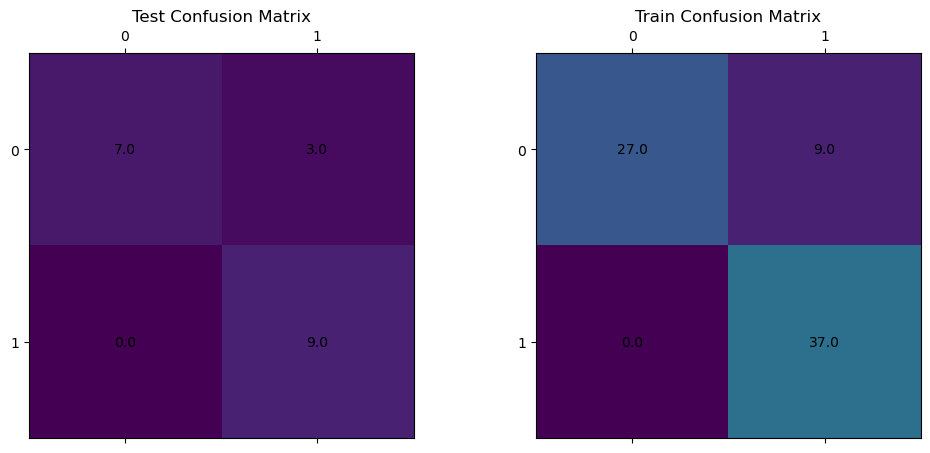
\includegraphics[width=0.9\textwidth]{resources/conf_svm_balanced.png}
            \caption{SVM on balanced}
            \label{fig:conf_svm_on_balanced}
        \end{figure}

        \newpage

        % image conf_svm_weighted.png

        \begin{figure}[h!]
            \centering
            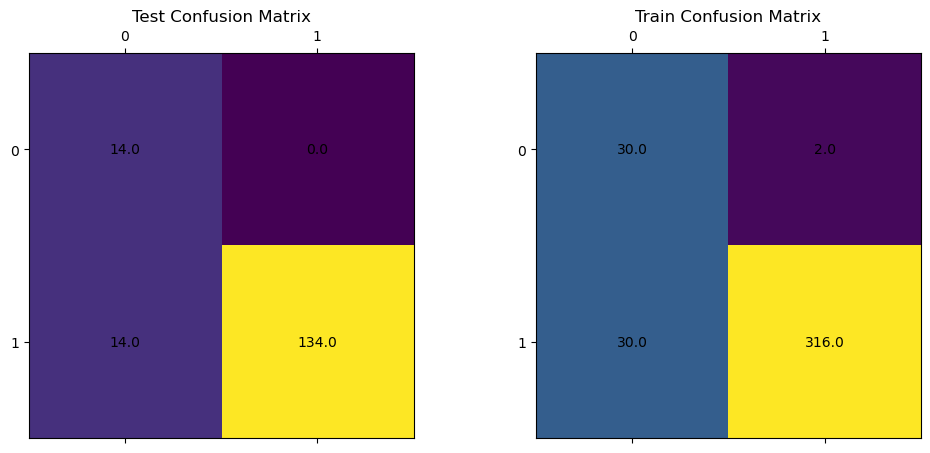
\includegraphics[width=0.9\textwidth]{resources/conf_svm_weighted.png}
            \caption{SVM weighted}
            \label{fig:conf_svm_weighted}
        \end{figure}

        % image conf_svm_weighted_on_balanced.png

        \begin{figure}[h!]
            \centering
            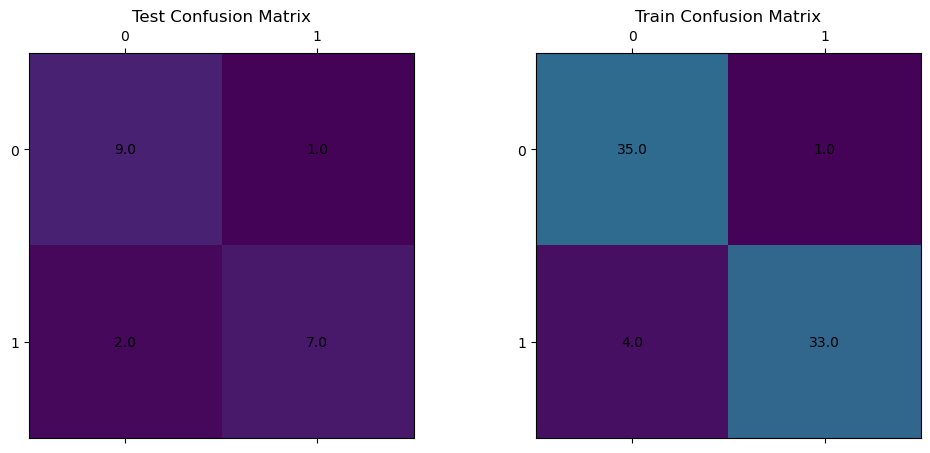
\includegraphics[width=0.9\textwidth]{resources/conf_svm_weighted_balanced.png}
            \caption{SVM weighted on balanced}
            \label{fig:conf_svm_weighted_on_balanced}
        \end{figure}

        \newpage

        % image conf_nn_baseline.png

        \begin{figure}[h!]
            \centering
            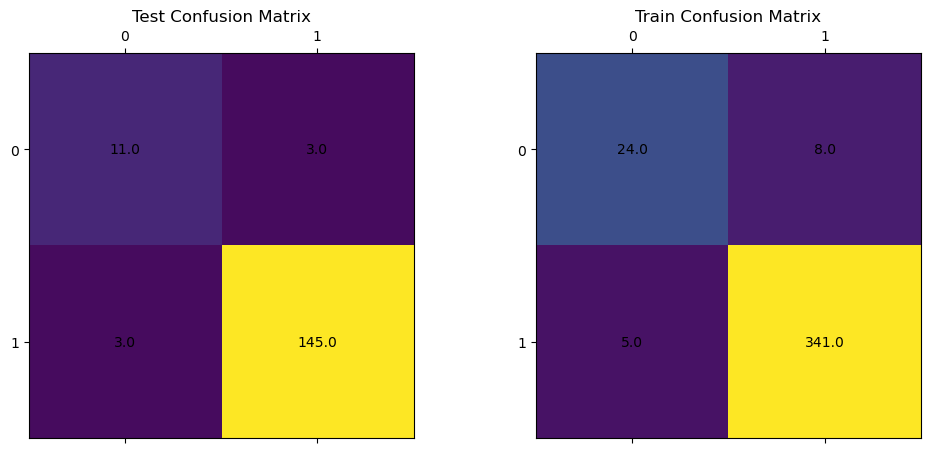
\includegraphics[width=0.9\textwidth]{resources/conf_nn_baseline.png}
            \caption{NN}
            \label{fig:conf_nn_baseline}
        \end{figure}

        % image conf_nn_baseline_on_balanced.png

        \begin{figure}[h!]
            \centering
            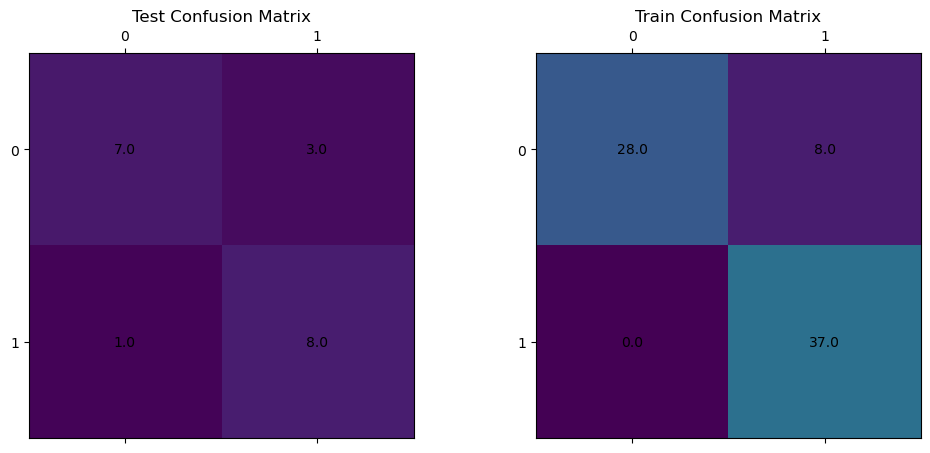
\includegraphics[width=0.9\textwidth]{resources/conf_nn_baseline_balanced.png}
            \caption{NN on balanced}
            \label{fig:conf_nn_baseline_on_balanced}
        \end{figure}

        \newpage

        % image conf_nn_biased.png

        \begin{figure}[h!]
            \centering
            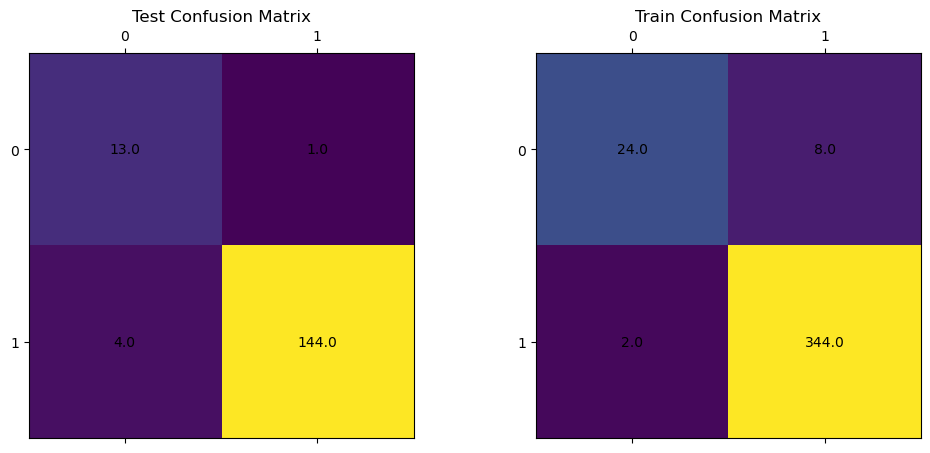
\includegraphics[width=0.9\textwidth]{resources/conf_nn_biased.png}
            \caption{NN biased}
            \label{fig:conf_nn_biased}
        \end{figure}

        % image conf_nn_biased_on_balanced.png

        \begin{figure}[h!]
            \centering
            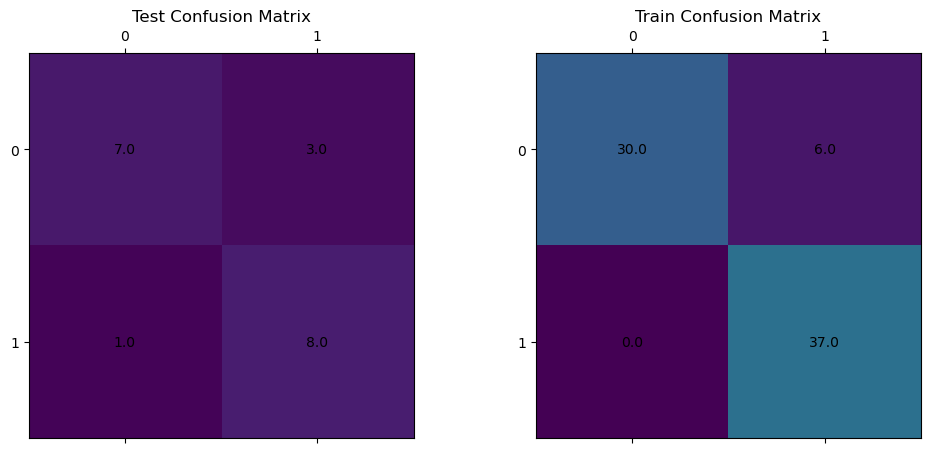
\includegraphics[width=0.9\textwidth]{resources/conf_nn_biased_balanced.png}
            \caption{NN biased on balanced}
            \label{fig:conf_nn_biased_on_balanced}
        \end{figure}

        \newpage

        % image conf_nn_weighted.png

        \begin{figure}[h!]
            \centering
            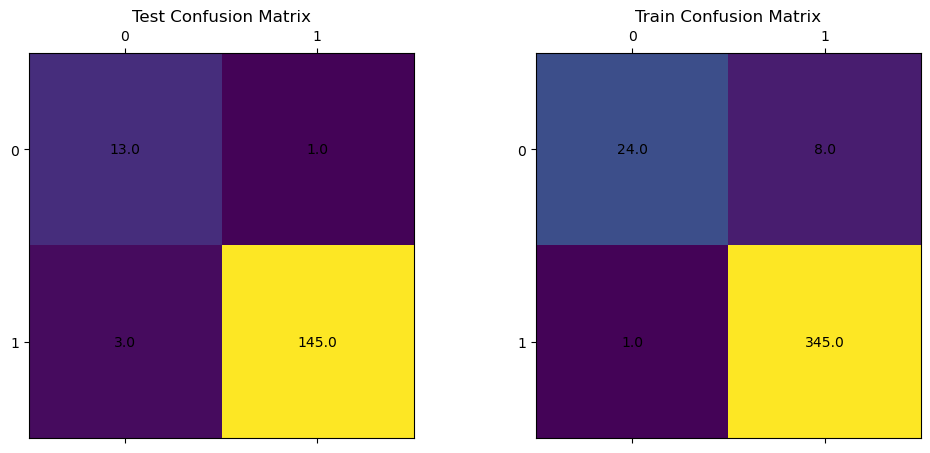
\includegraphics[width=0.9\textwidth]{resources/conf_nn_weighted.png}
            \caption{NN weighted}
            \label{fig:conf_nn_weighted}
        \end{figure}

        % image conf_nn_weighted_on_balanced.png

        \begin{figure}[h!]
            \centering
            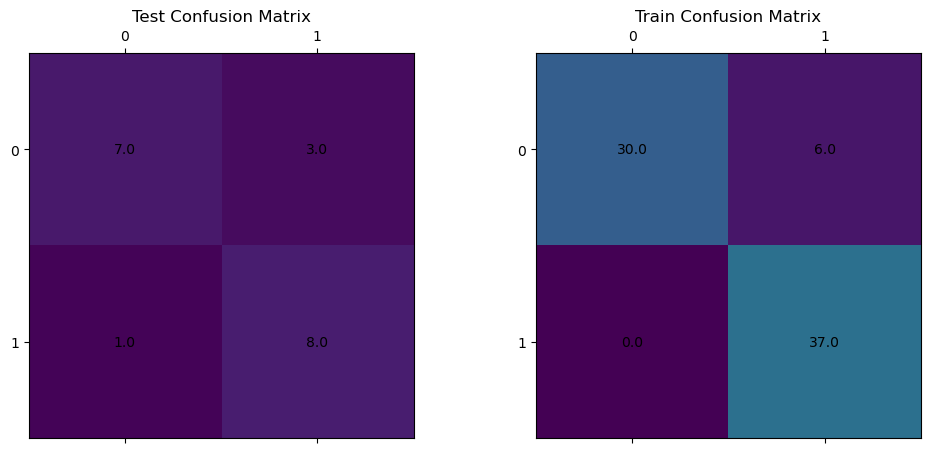
\includegraphics[width=0.9\textwidth]{resources/conf_nn_weighted_balanced.png}
            \caption{NN weighted on balanced}
            \label{fig:conf_nn_weighted_on_balanced}
        \end{figure}
        
        \newpage
        \subsection{Macierze pomyłek opis}
        Należy zauważyć że modele bardzo często różnią się predukcją jednej/dwóch próbek. Na podstawie tych 
        danych można znaleść kilka dobrych modeli
        
        \textbf{\code{SVM}} radzi sobie dobrze uzyskując całkiem zadawalające wyniki, 
        ale jest bardzo wrażliwy na zmiany w danych. Wersja z dostosowanymi wagami próbek również radzi sobie 
        najlepiej przy danych 50/50.

        \textbf{\code{NN}} radzi sobie w tym problemie bardzo dobrze i jest wstanie bez przetrenowania 
        (utzymuje się na train i val) uzyskać bardzo wysoki wskaźnik $r^2$. Najlepszym modelem ze wszystkich 
        jest właśnie sieć która posiada wagi dostosowane do ilości próbek, uzykuje $r^2$ na poziomie prawie $0.70$ i to na 
        wszystkich zbiorach! W zależności od oczekiwanych wyników można wybrać \textbf{\code{Weighted SVM}} ponieważ ilość 
        fałszywie pozytywnych i fałszywie negatywnych odpowiedzi są do siebie zbliżone dla zbiorów 
        testowych i zbalansowanych.
        
        \newpage
        
        \section{Krzywe uczenia}

        \begin{figure}[h!]
            \centering
            \subfloat[\centering prc]{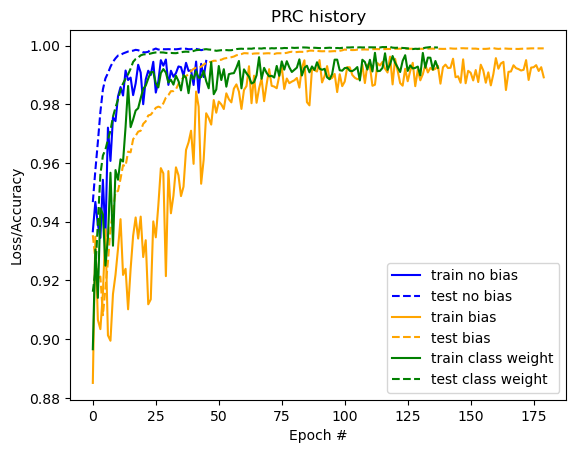
\includegraphics[width=0.5\textwidth]{resources/nn_learningcurve_prc.png}}
            \subfloat[\centering recall]{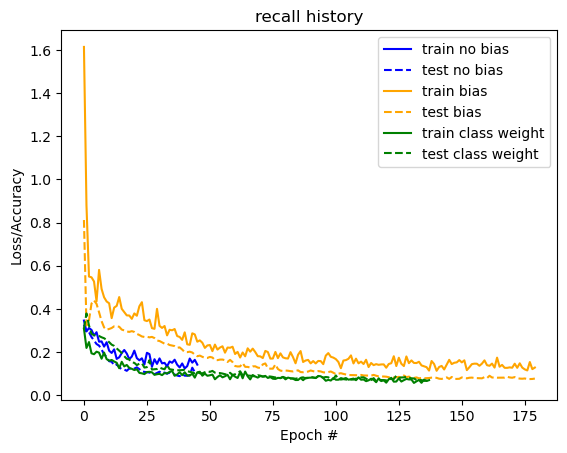
\includegraphics[width=0.5\textwidth]{resources/nn_learningcurve_recall.png}}
            \caption{Krzywe uczenia}
            \label{fig:learning_curves_prc}
        \end{figure}
        
        Krzywe uczenia są dość obiecujące, ze względu na ostrą regularyzacje modelu przy uczeniu, błąd dla
        zbioru treningowego jest wyższy od zbioru testowego. A Błąd dla zbioru testowego bardzo szybko osiąga 
        zbieżność co oznacza że model jest zmuszony szukać zależności w danych.

    \section{Podsumowanie}

    Uczenie modeli na taich danych jest okrutne i wymaga dużo strojenia hiperparametrów. Chociaż z odpowiednimi technikami
    jest się w stanie uzyskać dobre wyniki. W tym przypadku najlepszym modelem jest sieć neuronowa z dostosowanymi wagami
    pozwlającymi uczyć się na niezbalansowanych zbiorach danych lub SVM. 

    Dużym wyzwaniem jest przetestowanie modeli ponieważ nie ma możliwości uzyskania dokładnych wyników 

    Dokładne wyniki dostępne są w notatniku. 
    
    \newpage

    \begin{thebibliography}{9}
    \bibitem{} \href{http://karpathy.github.io/2019/04/25/recipe/#2-set-up-the-end-to-end-trainingevaluation-skeleton--get-dumb-baselines}{set-up-the-end-to-end-trainingevaluation-skeleton--get-dumb-baselines}
    \bibitem{} Uczenie maszynowe z użyciem Scikit-Learn i Tensorflow Aurelien Geron Wydanie inicjalizacja
    \bibitem{} \href{https://scikit-learn.org/stable/model_selection.html#model-selection}{scikit-learn model selection}

\end{thebibliography}
    
\end{document}